\chapter{Návrh}\label{chap:design}
Tato kapitola se bude zabývat návrhem sestavy technologií, které se budou využívat pro realizaci \gls{api}.

\section{Model vývoje}\label{sec:development_model}
Jako model vývoje byl použit klasický vodopádový model \figureref{fig:waterfall}, který sice v praxi není úplně realistický, ale je dobrým základem pro popis vývojového procesu modelové hry. Používá se primárně v situacích, kdy je definice projektu jasná a je zřejmý i cíl, kdy je dost času pro vývoj a kdy je možné všechny fáze vývoje pečlivě naplánovat, aby se minimalizovaly chyby.

První vlastností tohoto modelu je \textbf{sekvenční přístup}, neboť nemožnost pracovat na další části vývoje, dokud přechozí není plně dokončena. Další z vlastností je \textbf{řízení dokumentací}, kdy se všechny fáze vývoje musí pečlivě dokumentovat, aby se minimalizoval čas strávený zpětnou analýzou provedených kroků. \textbf{Kontrola kvality} je při tomto modelu důležitá, neboť chyby, které by se mohly vyskytnout v prvotních fázích vývoje, se mohou nepříjemně projevit a vývoj zkomplikovat. S tím se pojí i \textbf{přísné plánování}, kdy je nutné všechny fáze vývoje pečlivě naplánovat a zvážit možná rizika, která by mohla vzniknout.\cite{geeksForGeeks:waterfall}

Tímto modelem jsme se snažili řídit, ale i přes důkladné promyšlení použitých návrhů se muselo v průběhu pár drobností upravovat. 

\begin{figure}[!ht]
    \centering
    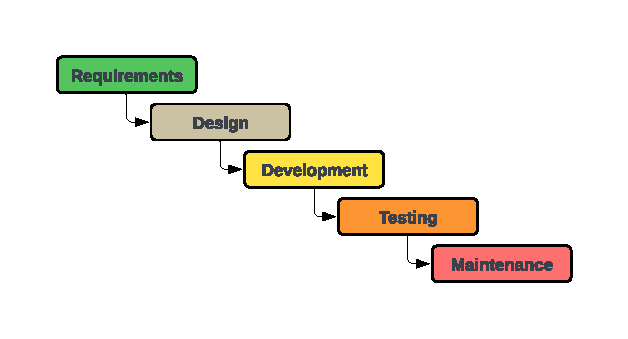
\includegraphics[width=0.8\textwidth]{figures/impl/API Implementation - waterfall model.pdf}
    \caption{Vodopádový model vývoje}\label{fig:waterfall}
\end{figure}

Ve fázi \textbf{požadavků} byly vzneseny nápady, jak samotná hra bude fungovat, jaké mechaniky použijeme a jakým způsobem by je bylo možné implementovat, přičemž nám vystačil pouze dokument s nápady a požadavky. Taktéž si zde všichni ujasnili, jaké herní mechaniky budou použity a za jakých okolností. 

Ve druhé fázi \textbf{návrhu} probíhala tvorba upřesňujících diagramů, návrhu architektury a uživatelského rozhraní. V našem případě byly přesněji rozvrženy jednotlivé mechaniky a bylo blíže popsáno, co se od nich očekává. Zároveň byly aplikovány návrhové vzory, které byly vhodné pro daný problém, především ty týkající se \gls{restful api}.

Fáze \textbf{vývoje} zahrnuje implementaci návrhů a vytvoření funkčního programu. V této fázi se taktéž využívají unit testy, které ověřují funkčnost jednotlivých částí programu. 

Poslední fáze, \textbf{testování} a \textbf{údržba}, se starají o to, aby program byl bez chyb a aby jednotlivé programy fungovaly jako celek. Po tom, co byl projekt otestován a vše je funkční, jde do produkčního prostředí a už se pouze udržuje, což zahrnuje opravování drobných chyb, které nebyly odhaleny během testování.

\section{Spolupráce}\label{sec:collaboration}
Jak už několikrát bylo naznačeno, tato práce byla vytvářena v týmu, kde měl každý člen na starosti jinou hlavní komponentu.
\begin{itemize}[itemsep=0pt,parsep=0pt]
    \item \textbf{Herní systém} -- Barbora Kovalská
    \item \textbf{Backoffice} -- Pavel Mikula
    \item \textbf{Frontend} -- Miroslav Osoba
    \item \textbf{API} -- Martin Korotwitschka
\end{itemize}

V průběhu bylo třeba přidat i jiné komponenty, protože bez nich by nebylo zprovoznění hry jakožto celku možné, takže zvlášť na nich pracovalo více členů týmu. V raných fázích vývoje bylo taktéž běžné, že se jednotliví členové více podíleli i na ostatních úkonech. 

Komunikace v prvotních fázích vývoje probíhala především za pomocí nástroje Github Issues. Později, když už byla kostra projektu funkční, stačila interní komunikace.

\subsection{Rozdělení práce}\label{sec:collaboration:job_distribution}
Jak lze vidět na Obrázku \ref{fig:job_distribution}, každý člen týmu nesl zodpovědnost za svou část projektu. Toto rozdělení vycházelo především ze zadání prací. 

\begin{figure}[h]
    \centering
    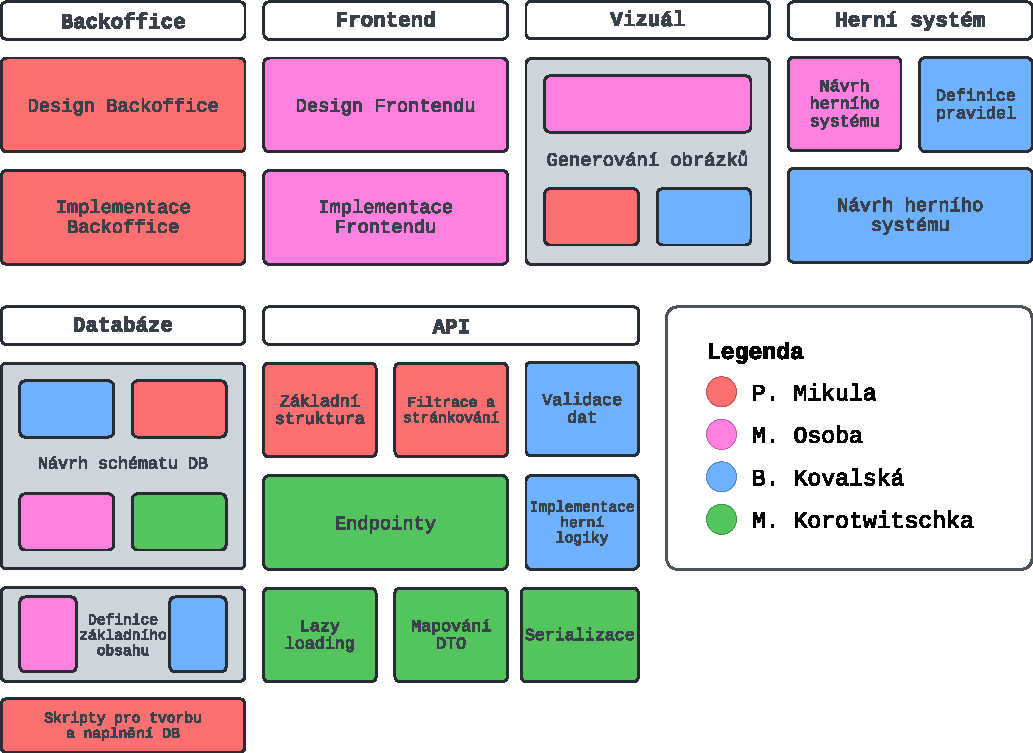
\includegraphics[width=\textwidth]{../../shared/diagrams/blocks.pdf}
    \caption{Rozložení práce v týmu}
    \label{fig:job_distribution}
\end{figure}

Pro přehlednost a verzování kódu byla vytvořena organizace na platformě GitHub \figureref{fig:gitOrg}, kde se vytvořily samostatné repozitáře pro každou část projektu. Taktéž se zde vedly \textit{Issues}, které zvlášť v prvotních fázích ulehčovaly vývoj a komunikaci.

\begin{figure}[H]
    \centering
    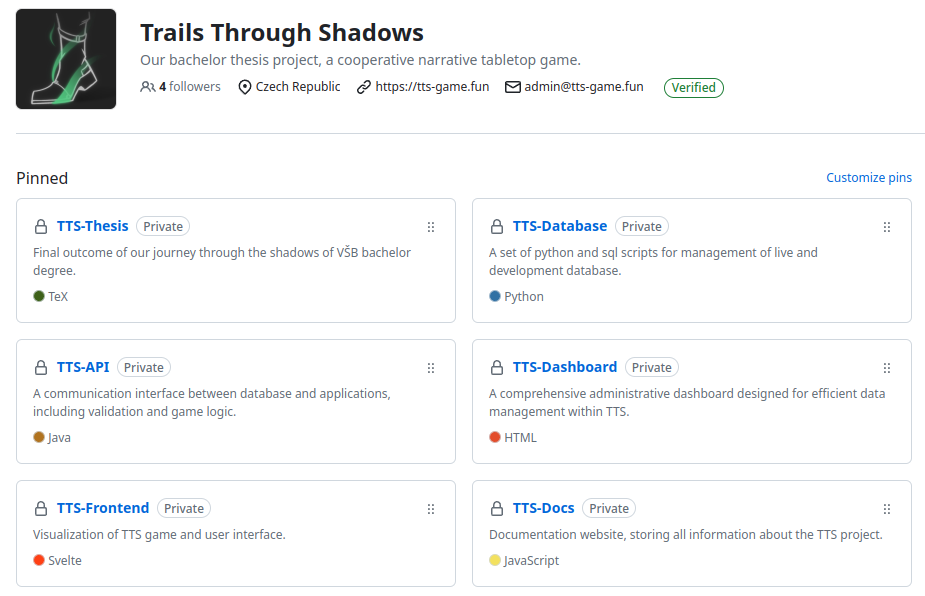
\includegraphics[width=\textwidth]{../../shared/figures/gitOrg.png}
    \caption{Organizace \textit{Trails Through Shadows} na platformě GitHub}
    \label{fig:gitOrg}
\end{figure}

Verzovací systém byl potřeba obzvlášť v případě API, na kterém pracovali primárně dva členové týmu. K ulehčení spolupráce zde bylo využito tzv. větví pro implementaci rozličných funkcionalit. Dokud nebyla kostra API hotová, nebylo takovéto rozdělování účinné a často se tak musely řešit konflikty.

Poté, co byla vytvořena kostra API, se začaly řádně využívat větve a jejich pravidla. Jako hlavní větev byla zvolena \textit{master}, na které byla vždy poslední stabilní verze, která byla nasazena na server. Další větev byla \textit{development}, na které se uchovávaly většinou funkční ale neotestované funkcionality. Ostatní větve se už v pozdější fázi vývoje nevyužívaly, protože každý vývojář pracující na tomto projektu měl svou vlastní složku, ve které pracoval, čímž bylo zabráněno konfliktům. Výše popsané strategii dělání větví a jejich následnému sloučení se říká \textit{Gitflow}.

\begin{figure}[H]
    \centering
    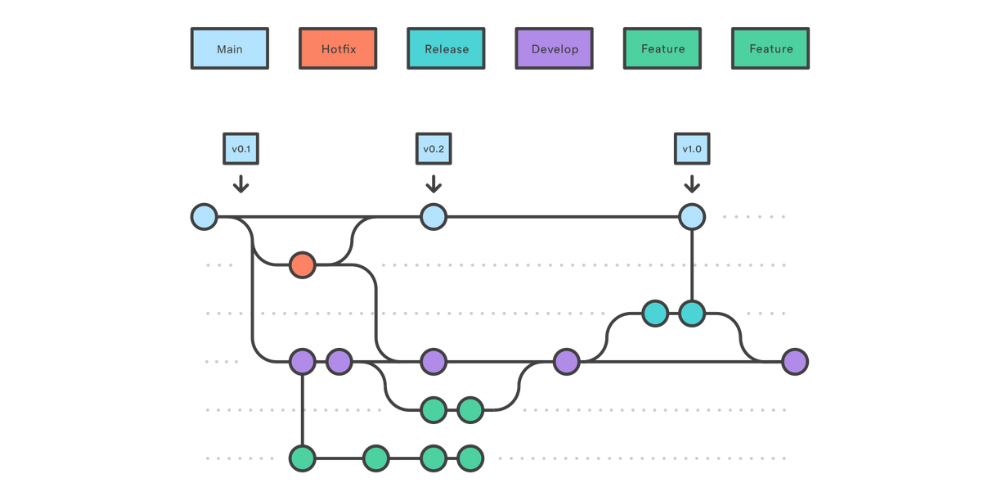
\includegraphics[width=\textwidth]{figures/impl/git-flow.png}
    \caption{Příklad \textit{Gitflow} workflow \cite{tilburgScienceHub:gitBranching}}
    \label{fig:gitflow}
\end{figure}

U repozitáře TTS-Thesis, kde byly uchovány texty všech našich prací, jsme používali Trunk-Based vývoj, kde se všechny akce se provádějí na hlavní větvi. Tento styl fungoval hlavně díky tomu, že každý měl svou vlastní složku, jejíž funkčnost nebyla na těch ostatních vůbec závislá. Díky tomu jsme mohli mít instantní nasazení vytvořeného PDF z \LaTeX ~souborů na webovou stránku.


\section{Databáze}\label{sec:database}
Návrh celého projektu byl započat vytvořením návrhu databáze. Na návrhu se podíleli všichni členové týmu \figureref{fig:job_distribution}, jelikož bylo nutné, aby všichni členové věděli, co a jak bude v databázi strukturované. Návrh probíhal za pomocí placeného nástroje \textit{dbdiagram.io}, kde se  všichni mohli podílet i online na tvorbě schématu v jeden časový moment. Tento nástroj taktéž podporuje export do řady SQL dialektů, mimo jiné i do MySQL, který jsme použili, protože databáze MariaDB používá stejnou syntaxi \sectionref{sec:data_storage}.

V kompletním ER diagramu databáze \figureref{fig:dix:database_schema} lze vidět jednotlivé rozdělení tabulek dle barvy do jednotlivých logických celků \figureref{fig:database_schema:block}[, zjedodušené blokové schéma]. Každá tabulka má v prvním sloupci zaznamenáno, zda se jedná o klíč, v druhém název atributu a ve třetím jeho datový typ. Z jednotlivých řádků je vidět závislost na ostatních tabulkách.

\begin{figure}[h]
    \centering
    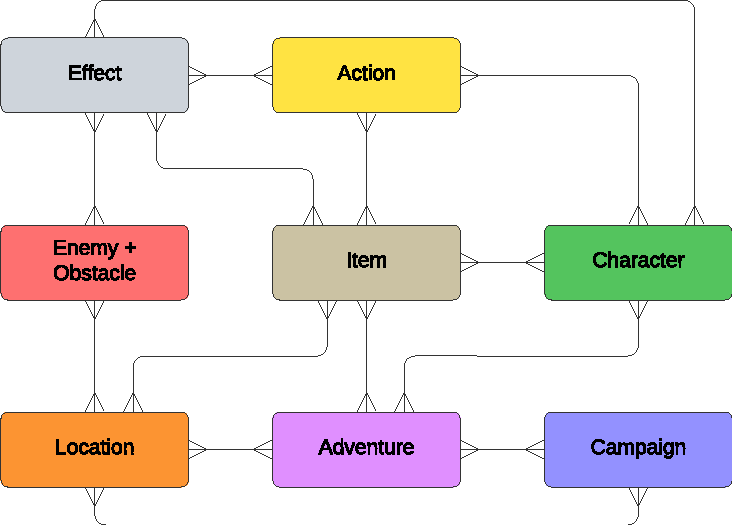
\includegraphics[width=0.5\textwidth]{../../shared/diagrams/er_macro.pdf}
    \caption{Zjednodušené databázové schéma podle logických celků}
    \label{fig:database_schema:block}
\end{figure}

Na prvním místě je žlutá sekce, která pojednává o \textbf{Akcích}. Základem je tabulka Action, která specifikuje, o jakou akci se jedná, zda o \textit{útok, pohyb, dovednost, obnovení karet} nebo o \textit{přivolání poskoka}. Akce samozřejmě může mít i více typů, a skoro každý typ akce může mít nějaký přídavný efekt.

Šedá sekce \textbf{Efekt} přidává spoustu modifikací, ať už jakékoli postavě jako například \textit{rezistenci na otrávení}, nebo modifikaci k útoku jako třeba \textit{krvácení}.

Zelená sekce se stará o \textbf{Postavu hráče}. Jako hlavní tabulka je zde \textit{Character}, která má vazbu na definici, o jakou postavu se bude jednat, neboli tabulky \textit{Třída} a \textit{Rasa}, podle kterých postava dostane své \textit{Akce}. Hráč má i inventář, ve kterém může mít jednotlivé předměty, které mu přidávají ať už statické bonusy nebo jednorázové výhody v boji.

Béžová sekce \textbf{Předmět} má na starosti \textit{Předměty} a jejich vazby na obchody, ve kterých se nacházejí. Předměty, jak již bylo zmíněno výše, přidávají hráči bonusy.

\textbf{Protivník a Překážka} jsou v červené sekci a specifikují protivníka nebo překážku v lokaci, ve které se bude bojovat. Jsou spojeny stejnou barvou, protože tyto dvě entity jsou si velice podobné, rozdíl je jen v tom, že jedna je dynamická a druhá statická.

Sekce \textbf{Lokace}, která je oranžová, specifikuje lokaci, na které bude probíhat bojová interakce. Základem je tabulka \textit{Location} která má relace na vstupní a výstupní hexagony, na protivníky a překážky, dveře a na části, ze kterých se tato lokace skládá. 

Jako poslední sekce je \textbf{Kampaň a Dobrodružství}, které spolu úzce souvisí, i přes to, že jsou zapsány jinou barvou (Kampaň modrá a Dobrodružství fialová). \textit{Kampaň} má příběh k dané lokaci, seznam \textit{dobrodružství} a seznam lokací, které jsou v rámci ní propojené. \textit{Dobrodružství} má seznam hráčů, kteří se účastní a seznam dostupných lokací.
